\begin{figure}
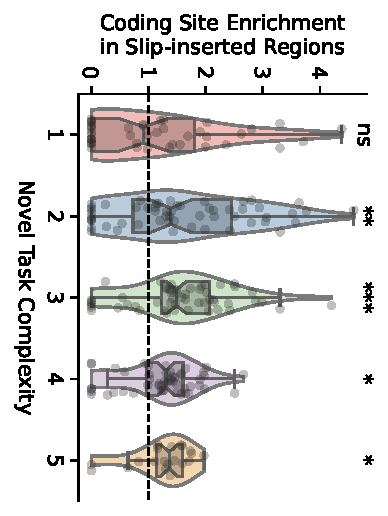
\includegraphics[
height=\linewidth,
angle=90
]{binder/binder/teeplots/density-norm=width+hue=components+viz=violinplot+x=components+y=is-task-coding-site+ext=.pdf}
\caption{%
  \textbf{Slip-duplicated sites are overrepresented among \textit{de novo} coding sites for complex traits.}
  \footnotesize
  Distributions compare median enrichment of coding sites for novel tasks in slip-duplicated regions, normalized to neutral expectation.
  Values greater than 1 indicate that coding sites of novel traits occur more often in slip-duplicated regions compared to their background frequency.
  Significance of deviation from null expectation median value of 1.0 is indicated with * ($p < 0.05$), ** ($p < 0.01$), or *** ($p < 0.001$) (one-tailed Wilcoxon signed-rank test).
} \label{fig:potentiation}
\end{figure}
